\chapter{Herramientas para trabajar con ARM}\label{ch:herramientas_arm}

En el capítulo anterior se discuten las razones para seleccionar la
arquitectura \ac{ARM}, en este capítulo discutiremos las herramientas
con las que se cuentan para trabajar con esta arquitectura y se plantea
la falta de un simulador dentro de éste conjunto de herramientas.


\section{Herramientas existentes}

Para generar código \ac{ARM} se necesita un ensamblador, y un
compilador en caso de querer escribir código de nivel más alto. 

Se evaluaron varias herramientas que existen actualmente, como:
\begin{itemize}
\item CrossWorks 
\item MDK-ARM
\item \ac{GCC}
\end{itemize}
Una de las herramientas más accesibles es la del \ac{GCC}, es
de licencia libre y es la herramienta que se usa por defecto en Linux. 

\ac{GCC} nos provee de las herramientas básicas que deseamos utilizar
que son:
\begin{itemize}
\item Ensamblador
\item Compilador de C
\end{itemize}
El \emph{ensamblador} es el componente que se encarga de convertir
el código ensamblador en código máquina, el ensamblador de \ac{GCC}
lo hace utilizando el formato binario \ac{ELF}, el cual especifica
en qué dirección de memoria se localiza y donde debe de estar
cuando se inicie la ejecución. El objetivo de este formato binario
es el de generar binarios más pequeños que indiquen al sistema
operativo como se debe de crear el proceso en memoria para su ejecución.

El \emph{Compilador} ejecuta una serie de tareas que tienen como objetivo
convertir el código C en ensamblador para posteriormente utilizar
al ensamblador para generar el binario, por ello también generará
programas \ac{ELF}. 


\section{Formato ELF}

\ac{ELF} es el formato común para archivos ejecutables, código objeto,
librerías compartidas y volcados de memoria. Fue desarrollado por
el UNIX System Laboratory (USL) y en 1999 fue elegido como el formato
estándar para archivos binarios en UNIX.

El formato \ac{ELF} tiene tres principales características por las
cuales en la actualidad se ha vuelto muy famoso entre diferentes sistemas
operativos y plataformas:
\begin{enumerate}
\item Flexible
\item Extensible
\item No esta ligado a un procesador o arquitectura en particular
\end{enumerate}
En la figura \ref{Flo:estructuraELF.png} se muestra la estructura
del formato \ac{ELF}, se compone de: 
\begin{itemize}
\item \ac{ELF}Header: contiene información importante del archivo \ac{ELF}
\item Program header table: describe cero o mas segmentos
\item Section header table: describe cero o mas secciones
\item Referencia a los datos dependiendo del numero de entradas del Program
header table y del Section header table.
\end{itemize}
%
\begin{figure}[!h]


\begin{centering}
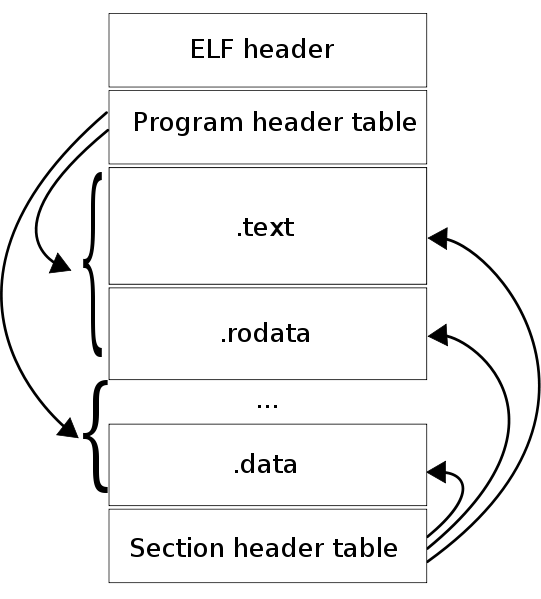
\includegraphics[scale=0.5]{img/estructuraELF}\caption{Estructura del formato ELF}
\label{Flo:estructuraELF.png}
\par\end{centering}


\end{figure}


Los segmentos contienen información importante para la ejecución del
programa mientras que las secciones contienen información importante
para la vinculación y reubicación.

Si desea mas información acerca de los tipos de datos que maneja un
\ac{ELF}, el contenido del \ac{ELF} Header y el contenido del Section
header table lo puede encontrar en el apéndice \ref{elfstruct.h}

Aún con estas herramientas hay algunos problemas en el desarrollo,
sobre todo por que las herramientas de software no modelan todas la
gama de productos que tiene la familia \ac{ARM}, la solución que
se plantea es el desarrollo de un simulador, con los mecanismos necesarios
para simular dispositivos externos.

Ésto podría llevar al desarrollo de un generador automático de simuladores,
donde se especifiquen los dispositivos externos y se genere un simulador
específico para ese microprocesador. Esto se discute con más detalle
en el capítulo \ref{ch:resultados}.



